\documentclass{standalone}

\usepackage{tikz}
\usetikzlibrary{decorations.pathreplacing,calligraphy}

\begin{document}
	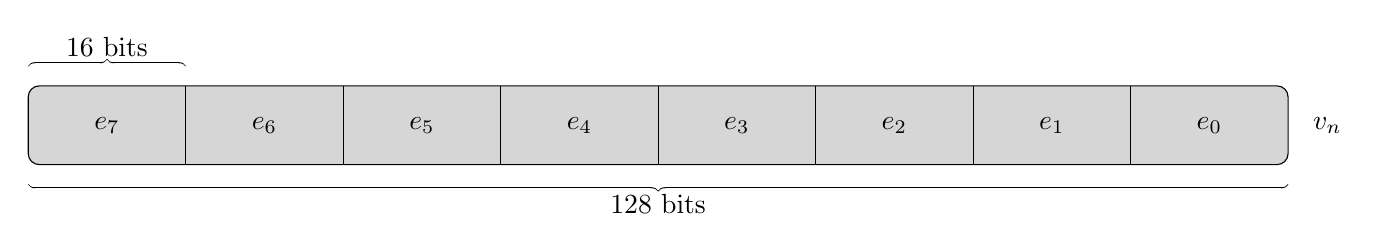
\begin{tikzpicture}
		\draw[fill=gray!32, rounded corners] (0, 0) rectangle (16, 1);
		\draw (2, 0) -- (2, 1);
		\draw (4, 0) -- (4, 1);
		\draw (6, 0) -- (6, 1);
		\draw (8, 0) -- (8, 1);
		\draw (10, 0) -- (10, 1);
		\draw (12, 0) -- (12, 1);
		\draw (14, 0) -- (14, 1);
		
		\node at (1, 0.5) {$e_{7}$};
		\node at (3, 0.5) {$e_{6}$};
		\node at (5, 0.5) {$e_{5}$};
		\node at (7, 0.5) {$e_{4}$};
		\node at (9, 0.5) {$e_{3}$};
		\node at (11, 0.5) {$e_{2}$};
		\node at (13, 0.5) {$e_{1}$};
		\node at (15, 0.5) {$e_{0}$};
		
		\draw [decorate, decoration = {calligraphic brace}] (0, 1.25) --  (2, 1.25);
		\draw [decorate, decoration = {calligraphic brace, mirror}] (0, -0.25) --  (16, -0.25); 
		
		\node at (1, 1.5) {16 bits};
		\node at (8, -0.5) {128 bits};
		
		\node at (16.5, 0.5) {$v_{n}$};
	\end{tikzpicture}
\end{document}